\chapter{Git (II) - Collaborating With Others}
\label{sec:git2}

\textit{Advanced Chapter}
\vspace{6mm}

The commands introduced in \cref{sec:ch3} is only enough for working alone, mainly the normal \texttt{git add .; git commit -m "message"; git push} procedure. Things are slightly more hectic when you have more than one person working together in the same repository concurrently. 

\section{The ideal situation}

Ideally, only one user should work on the project at a time. After someone has finished working, they push their code to GitHub. Then all other people would get the latest code from GitHub and download it to their local device using \texttt{git pull} before they start working on their part of the code. 

Note the distinction between \texttt{git pull} and \texttt{git clone} (see \cref{sec:gitclone}). \texttt{git clone} is to copy the repository to your local device, it is only used to download the code initially. \texttt{git pull} is used for subsequent downloads, which aims to update the local code with newest changes.

\begin{figure}[h]
\centering
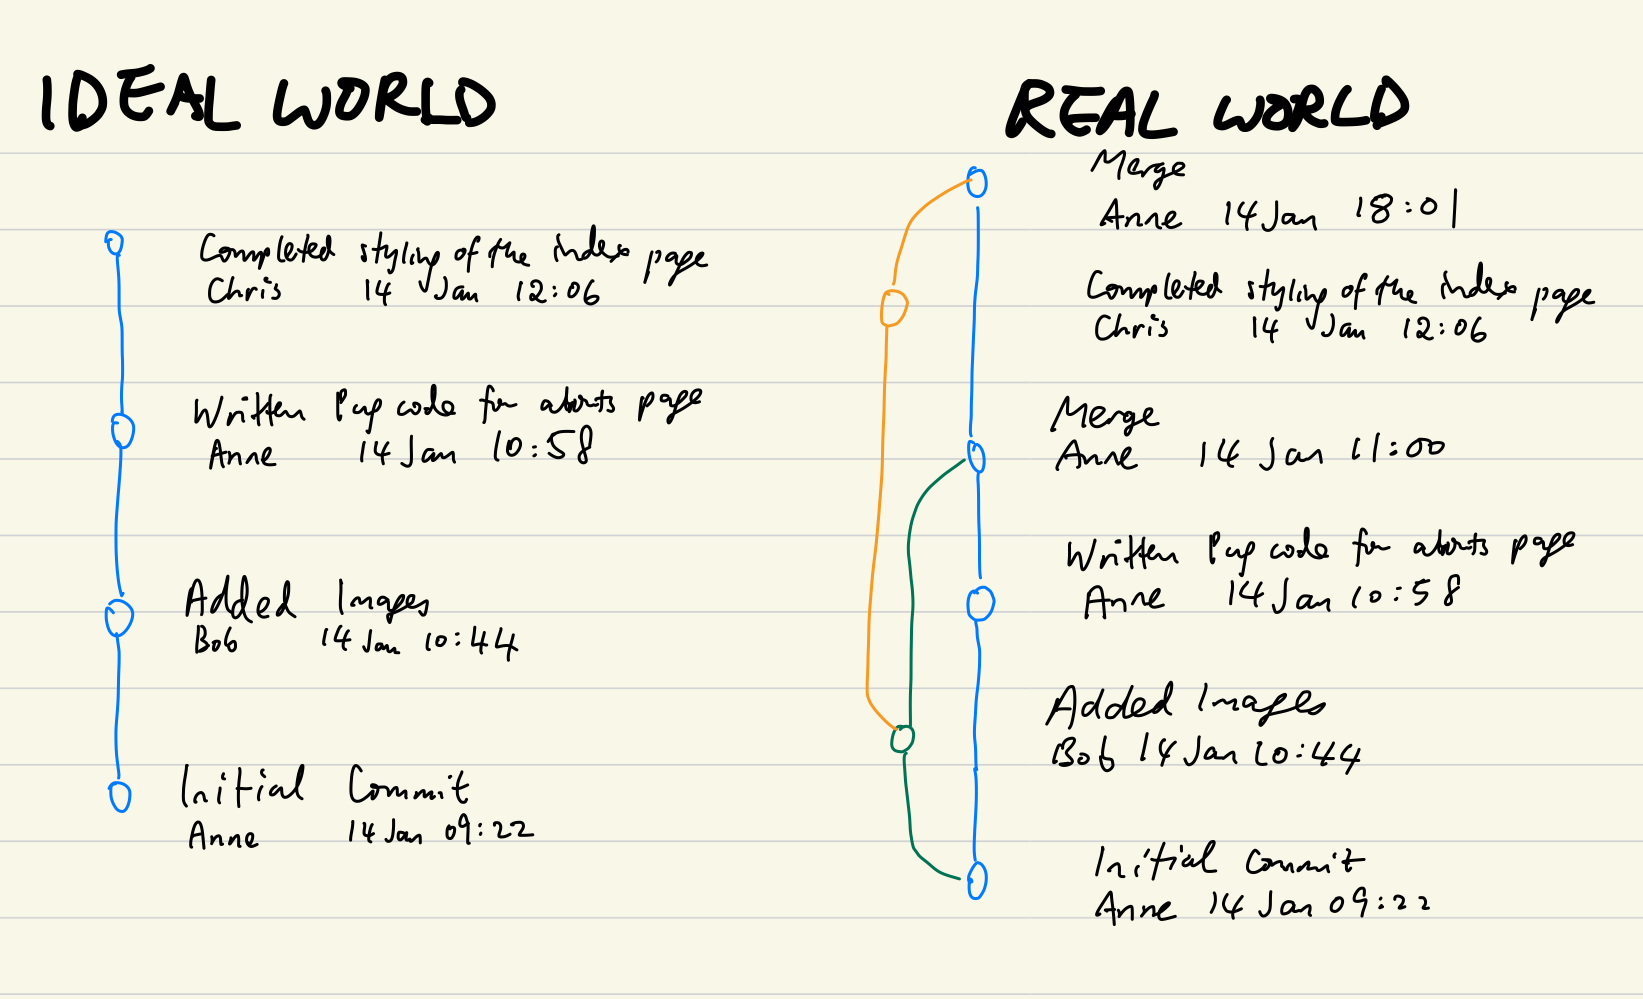
\includegraphics[width=15cm]{images/ch8-messy-git-world.png}
\caption{Messy world of Git}
\end{figure}

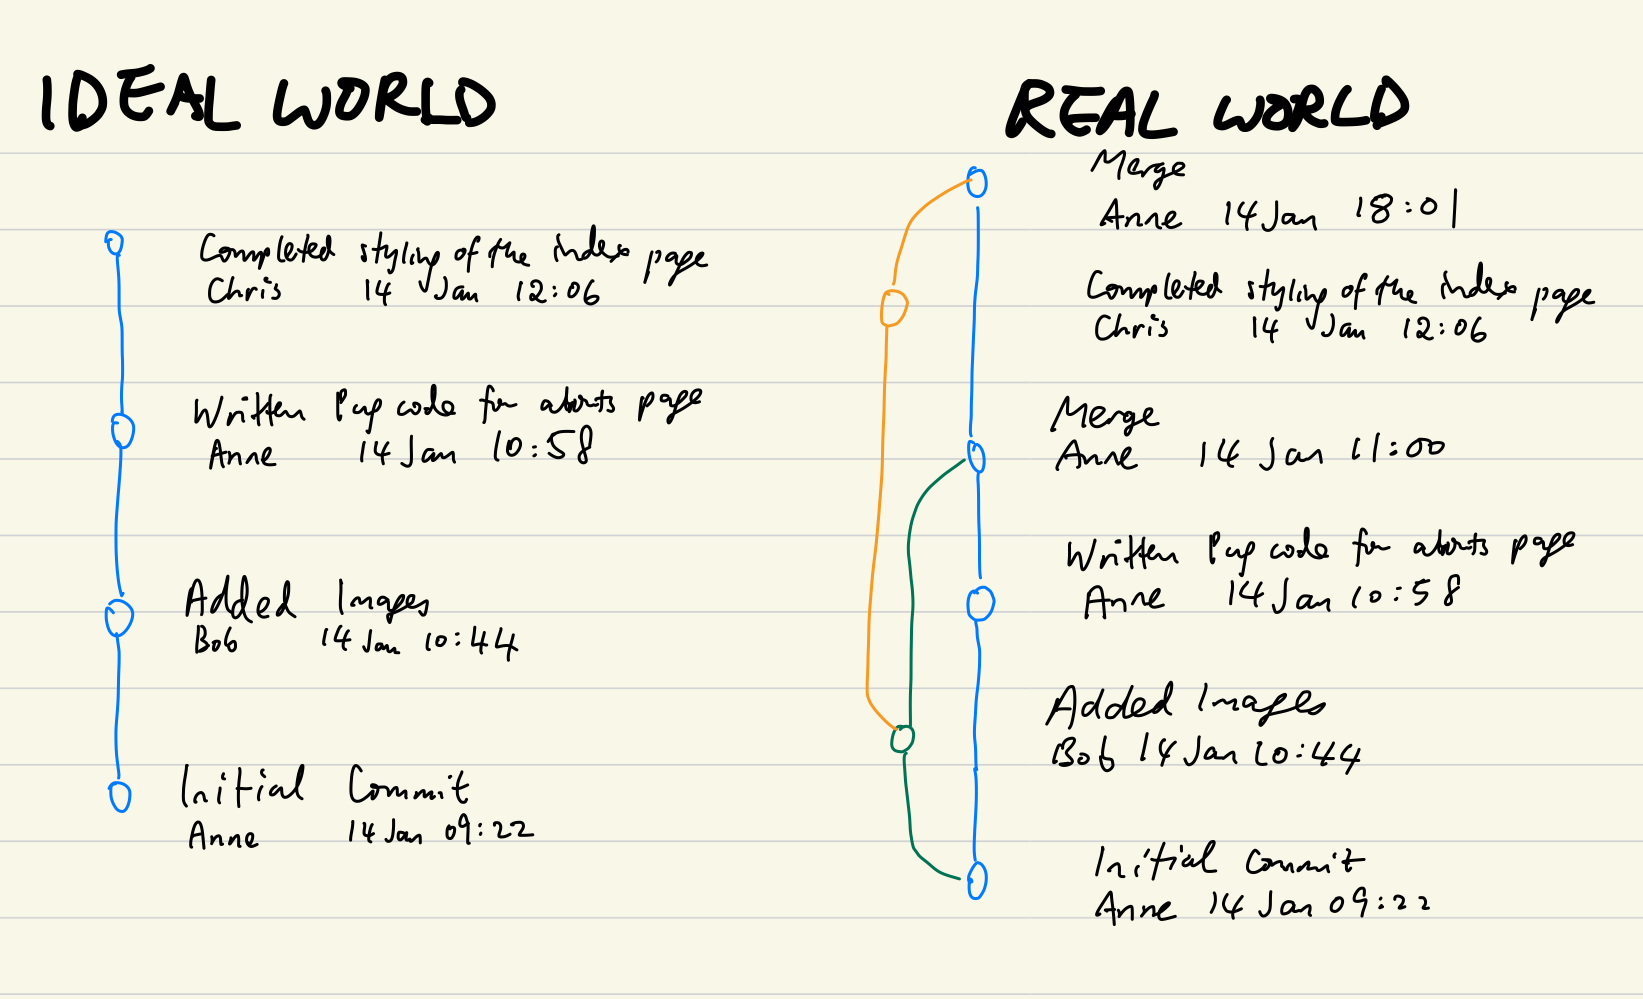
\includegraphics[width=15cm]{images/ch8-messy-git-world.png}

Of course, the real world is messier. We are greedy and we want multiple people work on the code at the same time. Or sometimes people simply forgot to \textbf{pull} (fancier word for download) the latest version of the code before they start working. We have to accept the fact that our \textbf{commit history} (fancier term for edit history) is not a straight line and diversions are unavoidable, just like our lives.\footnote{For fun: life is not a stright line \url{https://amandalinehan.com/life-is-not-a-straight-line/}} We will discuss git commands and techniques that can help you to work with different people in this chapter.

\section{Branching out}

We use branches to maintain different versions of the same project. 

\subsection*{\texttt{git checkout -b} and \texttt{git checkout}}

Creating a new branch using \texttt{git checkout -b} followed by the branch name you want. In the example below, we switched from main branch to our newly created beta branch. The newly created branch has the same contents as the branch you switched from.

To switch to an existing branch, we use \texttt{git checkout}. Note that for subsequent switches to the beta branch you don't need \texttt{-b} anymore, since the beta branch was created already it is now an existing branch.

\begin{lstlisting}[language=bash]
# KidProf in ~/code/git-tutorial on git:main x [22:38:58]
$ git checkout -b beta
Switched to a new branch 'beta'

# KidProf in ~/code/git-tutorial on git:beta x [22:39:12]
$ git checkout main
Switched to branch 'main'

# KidProf in ~/code/git-tutorial on git:main x [22:40:58]
$ git checkout beta
(Note no need -b here because beta is now an existing branch)
Switched to branch 'beta'

# KidProf in ~/code/git-tutorial on git:beta x [22:44:10]
\end{lstlisting}

In Git Bash and MacOS zsh (see \cref{sec:iterm} for set up) you can see the branch that you are currently in.

\subsection*{Example}

Switching between branches is now not particularly interesting, so let's now change that.

In the beta branch, we can try opening a random file and change its contents. Ideally mention something about the beta branch for easier recognition.

\begin{lstlisting}[language=pug]
//- app/templates/views/index.pug
extends ../layouts/default

block content
	.container
		h1 Welcome to Static Web!
		br
		p A very cool website.
		p This web is made for tutorial purposes.
		p Edits on beta branch in index page.
\end{lstlisting}

Commit your changes, using the three steps mentioned in \cref{sec:gcmsg}

\begin{lstlisting}[language=bash]
$ git add .
$ git commit -m "edits on beta branch"
$ git push
\end{lstlisting}

You might need to run \texttt{git push --set-upstream origin beta} instead because this is the first push of a new branch. 

Then let's switch back to main branch using \texttt{git checkout main}. Open the file you have modified in the beta branch, you will realise your edits are gone!

This is because we are now at the main branch, and you were making edits on the beta branch instead. Changes on one branch will not affect other branches, this is how you are able to maintain different versions of the same project.

We can make further experimentation with branches by making edits in the main branch also. I deliberately made edits to a different file, the reason will become apparent in the next section.

\begin{lstlisting}[language=pug]
//- app/templates/views/abouts.pug
extends ../layouts/default

block content
	.container
		p abouts page
		p Edits on main branch in abouts page.
\end{lstlisting}

\begin{lstlisting}[language=bash]
$ git add .
$ git commit -m "edits on main branch"
$ git push
\end{lstlisting}

Now you can switch back and forth between the two branches and see that the contents are different.

\begin{figure}[h]
\centering
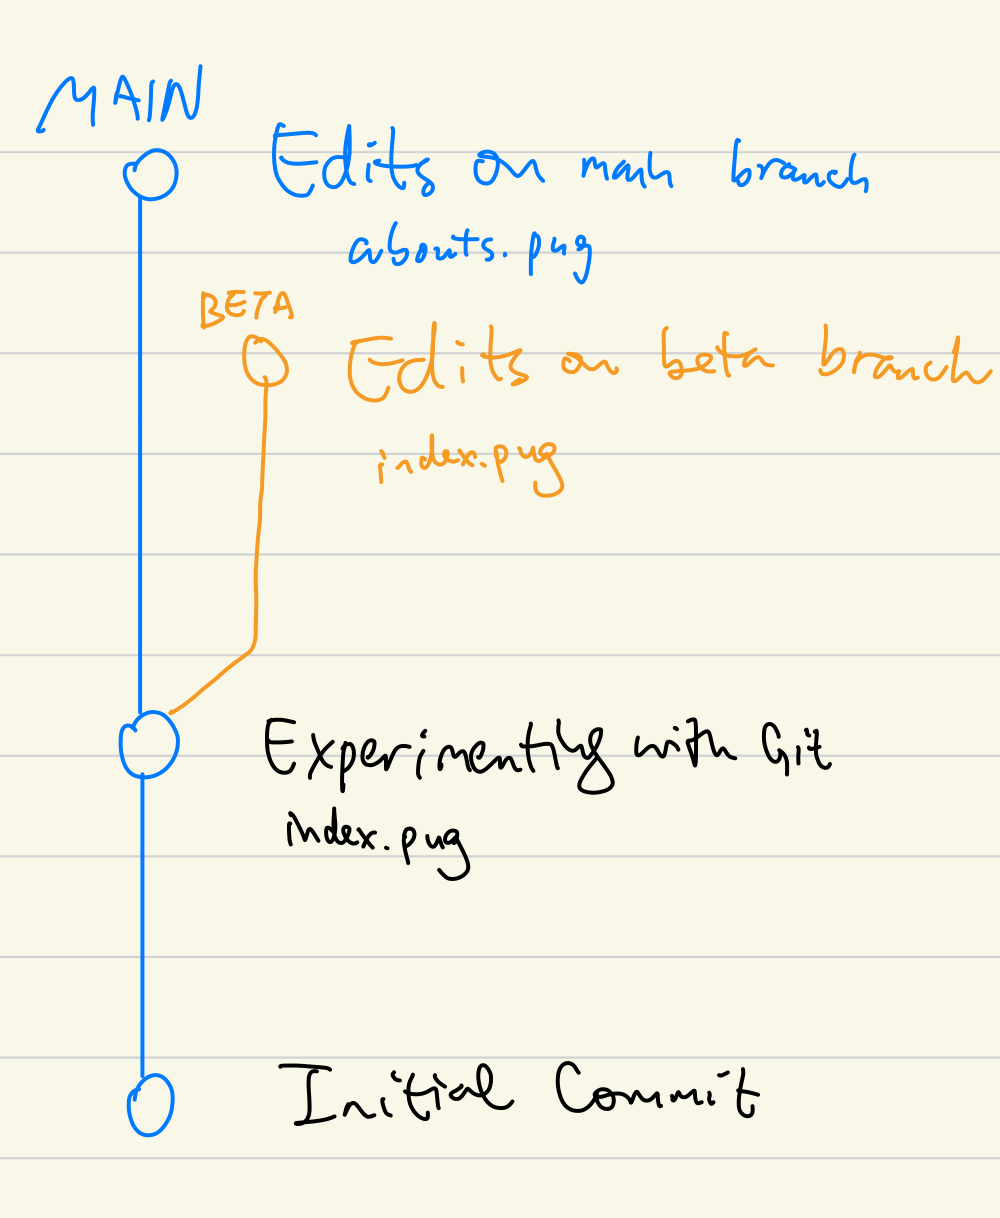
\includegraphics[width=7cm]{images/ch8-branching.png}
\caption{Visualising the two branches created}
\end{figure}

\subsection*{Uses of branches}
Yes we use branches to maintain different versions of the same project. The common practice will be each employee of a company work on their own branch named after their name (e.g. dev-kidprof), so that they can work on their own tasks without interfering with others.

However, we only want one version at the end, the version that you publish to the public. To achieve this, the employees will \textbf{merge} their branches (see next section) back to the main branch. The main branch usually is the final product of the project and it should be relatively error free because all known issues should be resolved before merging code from other branches to the main branch.

\section{Merging}

\subsection{Merge Without Conflicts}

We will try to merge the beta branch into the main branch (i.e. apply the changes in beta branch to the main branch)

We can do so by first checking out to the main branch, the branch that you want to merge into.
\vspace{6mm}

\begin{lstlisting}[language=bash]
$ git checkout main
\end{lstlisting}

\vspace{6mm}
Then run the command \texttt{git merge}, to merge the beta branch into the main branch.

\vspace{6mm}\begin{lstlisting}[language=bash]
$ git merge beta
\end{lstlisting}
\vspace{6mm}

A command line text editor may pop up, we do not need to modify anything. So we can just type \texttt{:wq} then tap enter to quit the text editor and save. For more information on how to control the command line text editor, refer to \cref{sec:vim}.

When you check your code, your edits in both the index page and abouts page are there. :)

Finally, push our merge to GitHub with \texttt{git push}.
\vspace{6mm}

If you want your beta branch to obtain the updates from the main branch, we can do the same for beta branch, that is:
\vspace{6mm}

\begin{lstlisting}[language=bash]
$ git checkout beta
$ git merge main
$ git push
\end{lstlisting}

\begin{figure}[h]
\centering
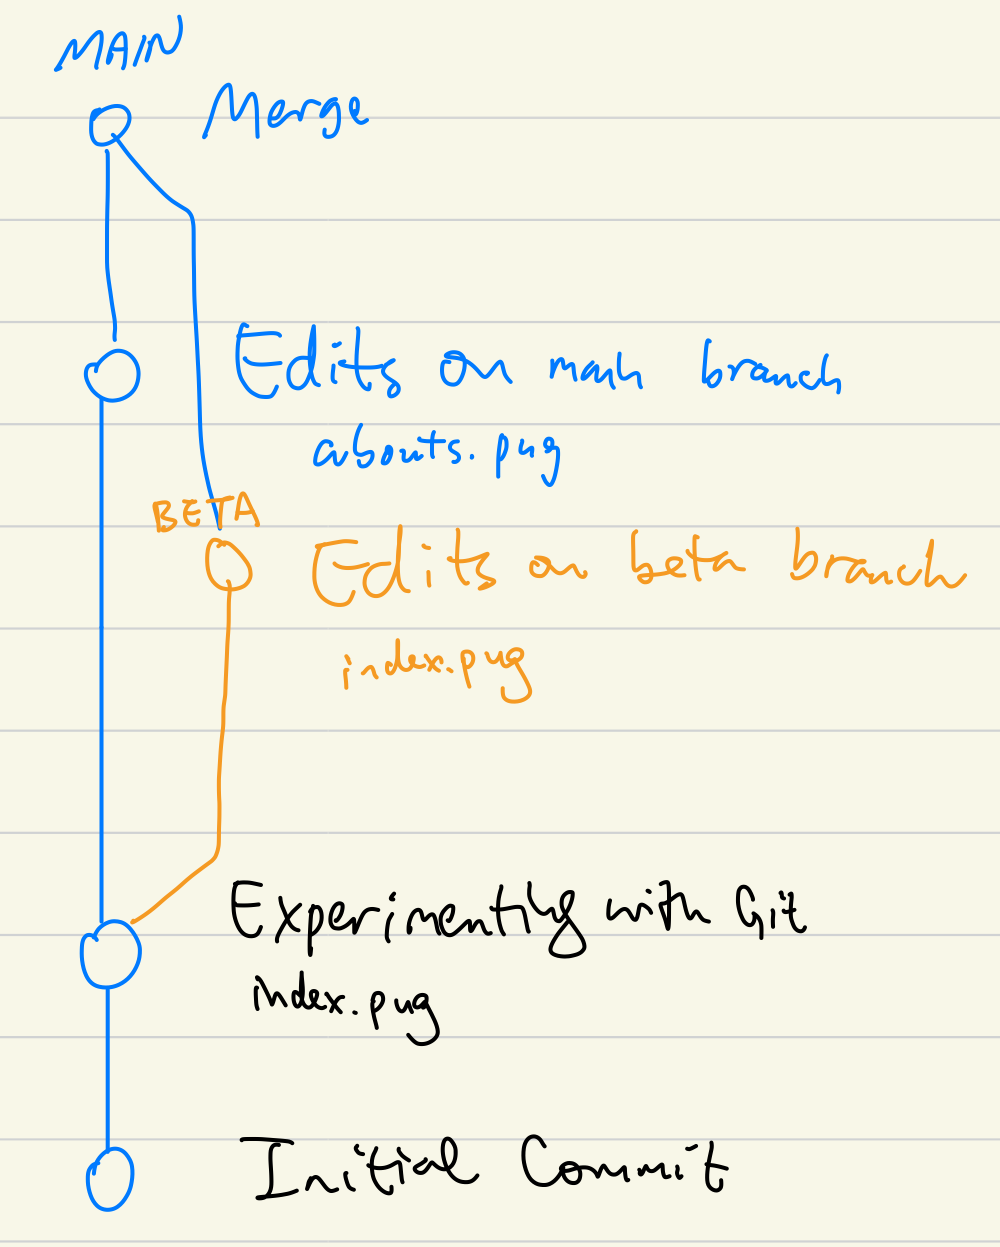
\includegraphics[width=7cm]{images/ch8-merge-safe.png}
\caption{Visualising the merge}
\end{figure}

\subsection{Merge Conflict}
\label{sec:mergeconflict}
The merge just now seems a bit too easy, that is because the two branches edited different files. The merging process would be more interesting when both branches edit the same part of the file. The following illustrates an example.
\vspace{6mm}

We first go to main branch and add a new line in \texttt{index.pug}.
\vspace{6mm}

\begin{lstlisting}[language=bash]
$ git checkout main
\end{lstlisting}

\begin{lstlisting}[language=pug]
//- app/templates/views/index.pug
...
p This web is made for tutorial purposes.
p Edits on beta branch in index page.
p New line on main branch.
\end{lstlisting}

\begin{lstlisting}[language=bash]
$ git add .
$ git commit -m "editing main branch again"
git push
\end{lstlisting}
\vspace{6mm}

Then we go to the beta branch and do the same. You will see the edits you have made just now and also the edits you have made for abouts page are missing, that is because we are in a different branch.
\vspace{6mm}

\begin{lstlisting}[language=bash]
$ git checkout beta
\end{lstlisting}

\begin{lstlisting}[language=pug]
//- app/templates/views/index.pug
...
p This web is made for tutorial purposes.
p Edits on beta branch in index page.
p New line on beta branch.
\end{lstlisting}

\begin{lstlisting}[language=bash]
$ git add .
$ git commit -m "editing beta branch again"
$ git push
\end{lstlisting}
\vspace{6mm}

Then we go back to main branch and try to merge beta branch into main branch.

\begin{lstlisting}[language=bash]
$ git checkout main

# KidProf in ~/code/git-tutorial on git:main o [23:28:42]
$ git merge beta
Auto-merging app/templates/views/index.pug
CONFLICT (content): Merge conflict in app/templates/views/index.pug
Automatic merge failed; fix conflicts and then commit the result.
\end{lstlisting}

When you open VS code, you may see the conflicting part of the code.
\begin{figure}[h]
\centering
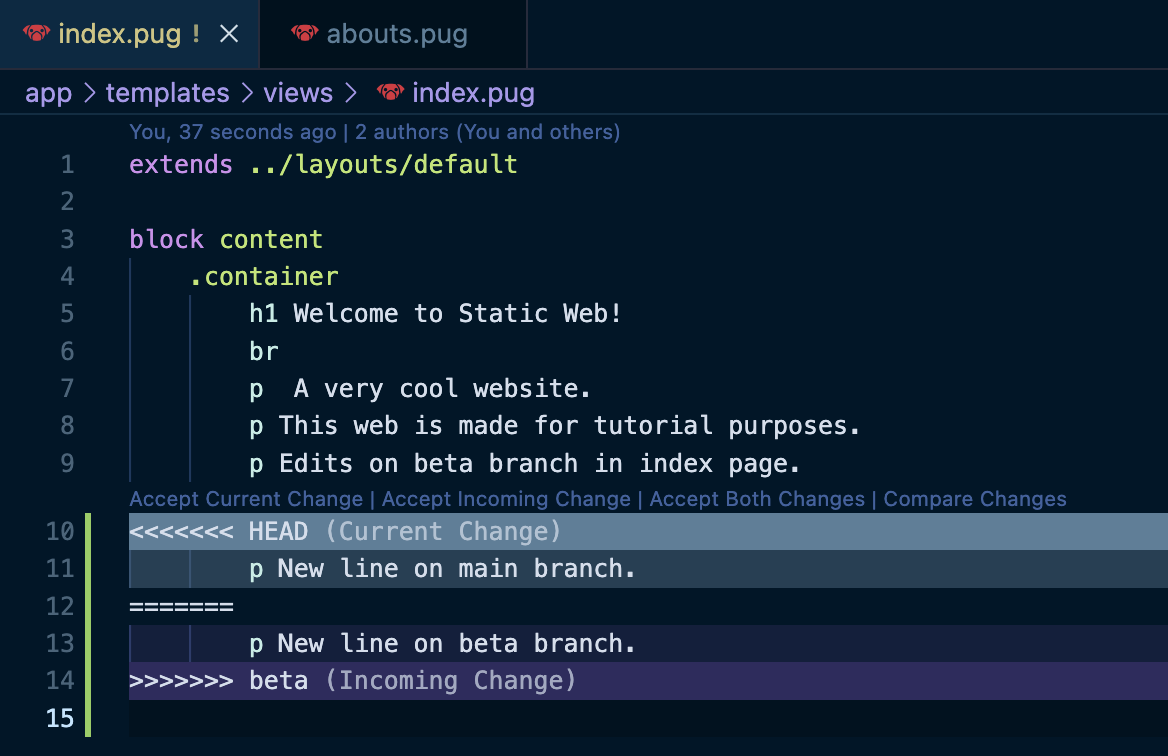
\includegraphics[width=12cm]{images/ch8-merge-conflict-vscode.png}
\caption{What sublime merge shows following the tutorial up to \cref{sec:mergeconflict}}
\end{figure}

\begin{lstlisting}[language=pug]
extends ../layouts/default

block content
	.container
		h1 Welcome to Static Web!
		br
		p  A very cool website.
		p This web is made for tutorial purposes.
		p Edits on beta branch in index page.
<<<<<<< HEAD
		p New line on main branch.
=======
		p New line on beta branch.
>>>>>>> beta
\end{lstlisting}

TODO: DNF

\begin{lstlisting}[language=bash]
$ git status
On branch main
Your branch is up to date with 'origin/main'.

You have unmerged paths.
  (fix conflicts and run "git commit")
  (use "git merge --abort" to abort the merge)

Unmerged paths:
  (use "git add <file>..." to mark resolution)
	both modified:   app/templates/views/index.pug
\end{lstlisting}

Finally, we just use the daily routine to push our merged code to GitHub. If no errors appear when running \texttt{git add .}, it means you have merged the code successfully.
\vspace{6mm}

\begin{lstlisting}[language=bash]
$ git add .
$ git commit -m "merge"
$ git push
\end{lstlisting}

\subsection*{When would there be a conflict when merging?}

When both branches modify the same part of the same file. (If two branches modify different parts of the file, there might not be one if Git recognises that the two edits are far away enough.)

\subsection*{Which changes should I choose when there is a conflict?}

It heavily depends on the situation! The Git tools provided by VS code may make you think only changes from one of the branch can be taken and we must discard the other, this is definitely not the case. The product of the merge should be what you want to be in your project finally. Maybe one of them is more updated, maybe you need to incorporate elements on both changes. For example, one branch may changed the indentation of a part of the code because they are now put in an if clause, while the other branch edited the contents of one line of the code. What you actually want is neither of them, but you need both the indentation change and content change.

\subsection{Merges due to edits on the same branch}

\section{Visualising}

Just a reminder, the visualisation tools introduced in \cref{sec:sublime} are super useful. It let's you see what's going on on different branches in a fashion that is similar to my illustrations.

\begin{figure}[h]
\centering
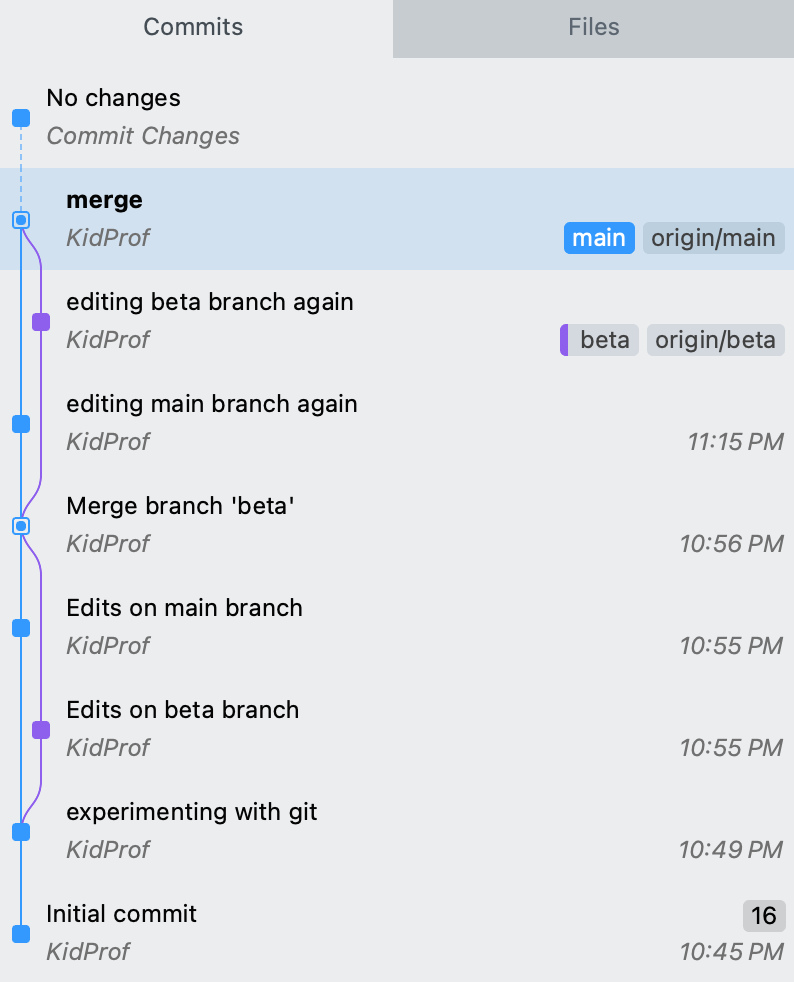
\includegraphics[width=7cm]{images/ch8-sublimemerge.png}
\caption{What sublime merge shows following the tutorial up to \cref{sec:mergeconflict}}
\end{figure}


\section{Stashing}

\textit{Of less importance}
\vspace{6mm}


